\documentclass[a4paper,12pt]{article}
  \usepackage{graphicx}
  \usepackage{indentfirst}
  \title{ImageNet Classification with Deep Convolutional Neural Networks}
  \author{Alex Krizhevsky \emph{et al.}}
  \date{2012}

\begin{document}
  \maketitle

\section{Preprocessing}

\begin{enumerate}
  \item
  Down-sample to fixed resolution $256 \times 256$.
  \item
  If rectangular, first rescale the image such that the shorter side is $256$, then crop out the central $256 \times 256$ patch.
  \item
  Subtract the mean activity over training set from each pixel.
\end{enumerate}

\section{Architecture}

The architecture of our network is summarized in Figure 1. It contains eight learned layers — five convolutional and three fully-connected. Below, we describe some of the novel or unusual features of our network’s architecture.

\begin{figure}[ht]
  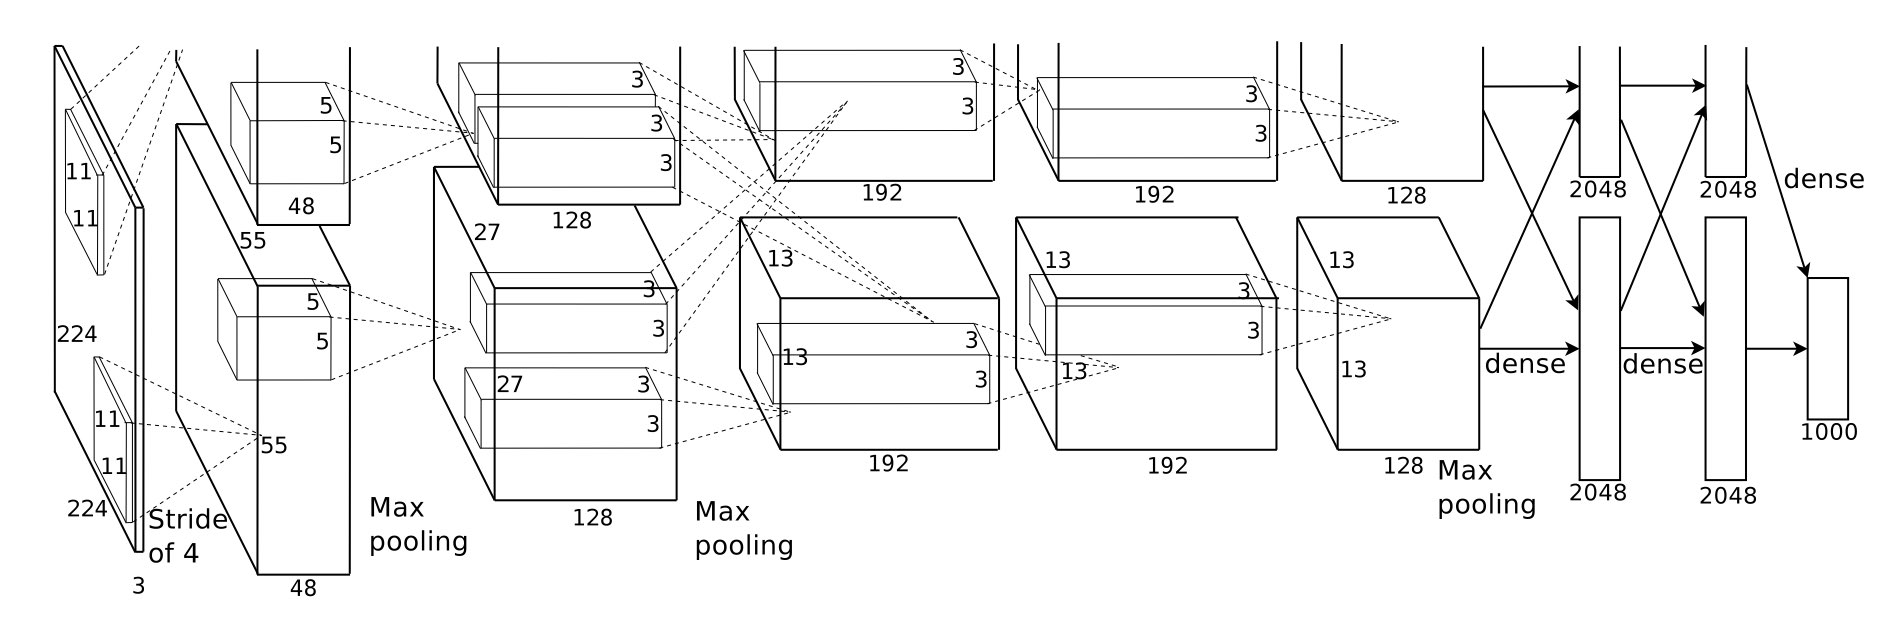
\includegraphics[width=\columnwidth]{figures/figure-1.jpg}
  \caption{An illustration of the architecture of our CNN.}
\end{figure}

\subsection{ReLU Nonlinearity}

Deep convolutional neural networks with ReLUs train several times faster than their equivalents with $\tanh$ units. Faster learning has a great influence on the performance of large models trained on large datasets.

\subsection{Local Response Normalization}

ReLUs have the desirable property that they do not require input normalization to prevent them from saturating. However, we still find that the following local normalization scheme aids generalization.

Denoting by $a^i_{x,y}$ the activity of a neuron computed by applying kernel $i$ at position $(x,y)$ and then applying the ReLU nonlinearity, the response-normalized activity $b^i_{x,y}$ is given by the expression

\[b^i_{x,y} = a^i_{x,y}/\left(k + \alpha\sum_{j=\max(0, i-n/2)}^{\min(N-1,i+n/2)}{(a^j_{x,y})^2}\right)^{\beta}\]

where the sum runs over $n$ “adjacent” kernel maps at the same spatial position, and $N$ is the total number of kernels in the layer. The constants $k$, $n$, $\alpha$, and $\beta$ are hyper-parameters whose values are determined using a validation set; we used $k = 2$, $n = 5$, $\alpha = 10^{-4}$, and $\beta = 0.75$.

This sort of response normalization implements a form of lateral inhibition inspired by the type found in real neurons, creating competition for big activities amongst neuron outputs computed using different kernels.

\subsection{Overlapping Pooling}

Suppose $s$ is the stride size and a pooling kernel is of size $z \times z$, we obtain overlapping pooling if we set $s < z$. This is what we use throughout our network, with $s = 2$ and $z = 3$.

\section{Reducing Overfitting}

\subsection{Data Augmentation}

We employ two distinct forms of data augmentation:

\begin{enumerate}
  \item Generating image translations and horizontal reflections.
  \item Altering the intensities of the RGB channels in training images.
\end{enumerate}

\subsection{Dropout}

We use dropout in the first two fully-connected layers. Without dropout, our network exhibits substantial overfitting. Dropout roughly doubles the number of iterations required to converge.

\section{Details of Learning}

We trained our models using stochastic gradient descent with a batch size of 128 examples, momentum of 0.9, and weight decay of 0.0005.

We initialized the weights in each layer from a zero-mean Gaussian distribution with standard deviation 0.01. We initialized the neuron biases in the second, fourth, and fifth convolutional layers, as well as in the fully-connected hidden layers, with the constant 1. This initialization accelerates the early stages of learning by providing the ReLUs with positive inputs. We initialized the neuron biases in the remaining layers with the constant 0.

We trained the network for roughly 90 cycles through the training set of 1.2 million images, which took five to six days on two NVIDIA GTX 580 3GB GPUs.

\section{Discussion}

Our results show that a large, deep convolutional neural network is capable of achieving record-breaking results on a highly challenging dataset using purely supervised learning.

\end{document}